\documentclass[__main__.tex]{subfiles}

\begin{document}

\qtitle{О}{12}
Плоская монохроматическая световая волна падает нормально на диафрагму с двумя узкими щелями, расстояние между которыми составляет $a$. На экране, находящемся на расстоянии $L$ от диафрагмы наблюдается интерференционная картина. На какое расстояние $x$ и в каком направлении произойдет смещение интерференционной картины, если одну щель покрыть стеклом толщины $d$ с показателем преломления $n$. Сформулируйте условия наблюдения интерференции.\\ 

\textbf{Условие наблюдения интерференции}.

Интерференция наблюдается при условии, что два световых источника являются когерентными. (Два источника света называются когерентными, если они имеют одинаковую частоту, угол между плоскостями колебаний световых векторов достаточно мал, разность фаз в точке наблюдения изменяется незначительно (менее чем на $\pi$) за время усреднения прибора наблюдения.\\

\begin{wrapfigure}{R}{0.4\linewidth}
	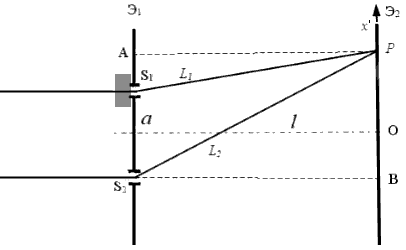
\includegraphics[width=1\linewidth]{img/o-12_1}{}
\end{wrapfigure}

 Из треугольника $S_1AP$ и учитывая наличие стекла найдем оптическую длину пути:
 $$L_1 = \sqrt{l^2 + \left(x' - \frac{a}{2}\right)^2} + nd$$
 Из треугольника $S_2AP$ найдем оптическую длину 
 $$L_2 = \sqrt{l^2  + \left(x' + \frac{a}{2}\right)^2}$$
 
 Так как $l \gg a, l \gg |x'|$, то используя формулу Тейлора (используем разложение $(1 + x')^\alpha = 1 + \alpha x'$, достаточно использовать первые два члена) получаем:
 
 $$L_1 = \sqrt{l^2 + \left(x' - \frac{a}{2}\right)^2} + nd = l\sqrt{1 + \left(\frac{x' - a/2}{l}\right)^2} \approx' l + \frac{(x' - a/2)^2}{2l} + nd$$
 Аналогично:
 $$L_2 \approx' l + \frac{\left(x' + a/2\right)^2}{2l}$$
 
 Найдем оптическую разность хода $\delta = L_1 - L_2 = x'a + nd$.\\

Максимумы наблюдаются при $\delta = m\lambda$, минимумы при $\delta = (m + 1/2)\lambda$.\\

Получаем, что максимумы будут появлятся при $x'_{max} = \frac{m\lambda - nd}{a}$, минимумы при $x'_{min} = \frac{(m + 1/2)\lambda - nd}{a}.$\\

Получаем, что смещение интерференционной картины $x = -\frac{nd}{a}$ (cмещается вниз)\\

\end{document}